% abtex2-modelo-artigo.tex, v-1.9.2 laurocesar
% Copyright 2012-2014 by abnTeX2 group at http://abntex2.googlecode.com/
%

% ------------------------------------------------------------------------
% ------------------------------------------------------------------------
% abnTeX2: Modelo de Artigo Acadêmico em conformidade com
% ABNT NBR 6022:2003: Informação e documentação - Artigo em publicação
% periódica científica impressa - Apresentação
% ------------------------------------------------------------------------
% ------------------------------------------------------------------------

\documentclass[
	% -- opções da classe memoir --
	article,			% indica que é um artigo acadêmico
	11pt,				% tamanho da fonte
	oneside,			% para impressão apenas no verso. Oposto a twoside
	a4paper,			% tamanho do papel.
	% -- opções da classe abntex2 --
	%chapter=TITLE,		% títulos de capítulos convertidos em letras maiúsculas
	%section=TITLE,		% títulos de seções convertidos em letras maiúsculas
	%subsection=TITLE,	% títulos de subseções convertidos em letras maiúsculas
	%subsubsection=TITLE % títulos de subsubseções convertidos em letras maiúsculas
	% -- opções do pacote babel --
	english,			% idioma adicional para hifenização
	brazil,				% o último idioma é o principal do documento
	sumario=tradicional
	]{abntex2}


% ---
% PACOTES
% ---

% Matemática
\usepackage{mathtools}

% ---
% Pacotes fundamentais
% ---
\usepackage{lmodern}			% Usa a fonte Latin Modern
\usepackage[T1]{fontenc}		% Selecao de codigos de fonte.
\usepackage[utf8]{inputenc}		% Codificacao do documento (conversão automática dos acentos)
\usepackage{indentfirst}		% Indenta o primeiro parágrafo de cada seção.
\usepackage{nomencl} 			% Lista de simbolos
\usepackage{color}				% Controle das cores
\usepackage{graphicx}			% Inclusão de gráficos
\usepackage{microtype} 			% para melhorias de justificação
% ---

% ---
% Altera as margens padrões
% ---
\setlrmarginsandblock{3cm}{3cm}{*}
\setulmarginsandblock{3cm}{3cm}{*}
\checkandfixthelayout
% ---

% ---
% Espaçamentos entre linhas e parágrafos
% ---

% O tamanho do parágrafo é dado por:
\setlength{\parindent}{0cm}

% Controle do espaçamento entre um parágrafo e outro:
\setlength{\parskip}{0.2cm}  % tente também \onelineskip

% Espaçamento 1.25
\linespread{1.25}
% ----
% Início do documento
% ----
\begin{document}


	\section*{Questão 2}

	\subsection*{Item a}
	Dado que
	$$f\left( x,y\right) =\begin{cases} \dfrac {xy^{2}} {x^{2}+y^{2}}, \quad \left( x,y\right) \neq \left( 0,0\right) \\ 0, \quad \left( x,y\right) =\left( 0,0\right) \end{cases} $$

	Para haver continuidade no ponto $\left( 0,0\right)$ a função acima deve satisfazer à seguinte condição
	$$\lim_{(x,y)\to(0,0) } f(x,y) = f(0,0) = 0$$

	Em outras palavras, para que haja continuidade no ponto considerado a asserção abaixo deverá ser verdadeira
	$$\lim_{(x,y)\to(0,0) } \dfrac {xy^{2}} {x^{2}+y^{2}} = 0$$

	Perceba que
	$$ -xy^{2} \leq \dfrac {xy^{2}} {x^{2}+y^{2}}\leq xy^{2}$$

	e que,
	$$ \lim_{(x,y)\to(0,0) } -xy^{2} = \lim_{(x,y)\to(0,0) } xy^{2} = 0  $$

	Portanto, pelo teorema do confronto, concluímos que
	$$\lim_{(x,y)\to(0,0) } \dfrac {xy^{2}} {x^{2}+y^{2}} = 0$$

	O que comprova a existência de continuidade no ponto considerado

	\subsection*{Item b}
	A derivada parcial da funcão em questão em relação a variável $x$ pode ser dado por
	$$\dfrac {\partial f} {\partial x} = \lim_{\Delta x \to 0 } \dfrac {f(\Delta x, 0 ) - f(0 , 0)}{\Delta x} = \dfrac {\Delta x \cdot 0} {x^2+0} = 0$$

	Analogamente para a variável $y$
	$$\dfrac {\partial f} {\partial y} = \lim_{\Delta y\to 0 } \dfrac {f(0 , \Delta y) - f(0 , 0)}{\Delta y} = \dfrac {0 \cdot \Delta y^2} {0+ \Delta y^2} = 0$$

	\subsection*{Item c}
	A diferenciabilidade de uma função será comprovada desde que afirmação

	$$\dfrac {E( x_0 + \Delta x, y_0 + \Delta y)} {||(\Delta x, \Delta y)||} = 0$$

	seja verdadeira.

	Neste caso $E( x_0 + \Delta x, y_0 + \Delta y)$ representa o que chamamos de "função erro".
	Seu valor é dado por

	$$E( x_0 + \Delta x, y_0 + \Delta y) =  f( x_0 + \Delta x, y_0 + \Delta y)  - f(x_0, y_0) - \dfrac {\partial f} {\partial x} \Delta x - \dfrac {\partial f} {\partial y} \Delta y $$

	Já $||(\Delta x, \Delta y)||$ pode ser dado por

	$$||(\Delta x, \Delta y)|| = (\Delta x^2 + \Delta y^2)^{1/2}$$

	Aplicando os dados que já temos à função erro,

	$$E( x_0 + \Delta x, y_0 + \Delta y) = \dfrac{\Delta x \cdot \Delta y^2}{\Delta x^2 + \Delta y^2} + 0 - 0 \cdot \Delta x - 0 \cdot \Delta y$$

	Poderemos afirmar que

	$$\dfrac {E( x_0 + \Delta x, y_0 + \Delta y)} {||(\Delta x, \Delta y)||} = \lim_{(\Delta x, \Delta y)\to(0,0) } \dfrac{\Delta x \cdot \Delta y^2}{(\Delta x^2 + \Delta y^2)^{3/2}} = 0$$

	Dessa forma comprovamos a difenciabilidade da função no ponto considerado.

	\section*{Questão 3}
	A região dado no enunciado por ser dada por


	\begin{figure}[!ht]
		\centering
		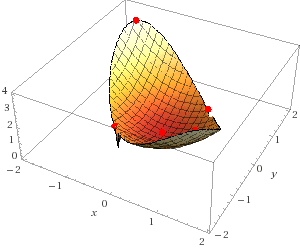
\includegraphics[width=0.5\linewidth]{/home/hellon/Dropbox/clientes/ana/images/3.png}
	\end{figure}

	A imagem acima revela que temos um mínimo global em $(0,0)$.

	Como sabemos que $f(x,y) = x^2 +y^2$ tem máximos e mínimos, e que a sua borda é dada por $g(x,y) = 5x^2+6xy+5y^2-8=0$, podemos afirma que

	$$\nabla f(x,y) =  - \lambda \nabla g(x,y) $$

	onde $\lambda$ corresponde a um \textit{multiplicador de lagrange}.

	Calculando os gradientes acima, chegamos a

	$$(2x,2y) = - \lambda  (10x+6 y, 6x+10 y)$$

	Chegamos assim ao seguinte sistema de equações

	$$\begin{cases} \left( 2+10\lambda \right) x+\left( 6\lambda \right) y=0\\ \left( 6\lambda \right) x+\left( 2+10\lambda \right) y=0 \\ \end{cases} $$

	Para que a nossa solução não tenha solução trivial ($x=0$ e $y=0$), o determinante dos coeficientes deve ser nulo, isto é

	$$
		\begin{vmatrix}
			2 + 10 \lambda & 6 \lambda \\
			6 \lambda & 2 + 10 \lambda
		\end{vmatrix}
		=
		0
	$$

	Ou seja
	$$(2+10 \lambda)^2 -36 \lambda^2 = 0$$

	No que resulta em $\lambda = -\frac{1}{2}$ e $\lambda = -\frac{1}{8}$


	\subsection*{i) Solução $\lambda = -\frac{1}{2}$}
	Para $\lambda = -\frac{1}{2}$ chegamos ao seguinte sistema de equações

	$$\begin{cases}  x + y = 0\\ 5x^2+6xy+5y^2-8=0\\ \end{cases} $$

	cuja soluções são dadas por $\left(-\sqrt{2}, \sqrt{2}\right)$ e $\left(\sqrt{2}, -\sqrt{2}\right)$.

	Para este conjunto de soluções temos, $f(x,y)=4$


	\subsection*{ii) Solução \lambda = -\frac{1}{8}}


	Para $\lambda = -\frac{1}{8}$ chegamos ao seguinte sistema de equações
	$$\begin{cases}  x - y = 0\\ 5x^2+6xy+5y^2-8=0\\ \end{cases} $$

	cuja soluções são dadas por $\left(-\dfrac{1}{\sqrt{2}}, -\dfrac{1}{\sqrt{2}}\right)$ e $\left(\dfrac{1}{\sqrt{2}}, \dfrac{1}{\sqrt{2}}\right)$.

	Para este conjunto de soluções temos, $f(x,y)=1$

	\subsection*{Conclusão}

	Temos os seguintes extremos $(0,0,0)$, $\left(-\dfrac{1}{\sqrt{2}},-\dfrac{1}{\sqrt{2}},1\right)$,
	$\left(\dfrac{1}{\sqrt{2}},\dfrac{1}{\sqrt{2}},1\right)$,
	$\left(-\sqrt{2}, \sqrt{2}, 4 \right)$, $\left(\sqrt{2}  -\sqrt{2}, 4 \right)$.	Sendo $(0,0,0)$ o mínimo global, $\left(-\sqrt{2}, \sqrt{2}, 4 \right)$ e $\left(\sqrt{2}, -\sqrt{2}, 4 \right)$
	os máximos globais.



	\section*{Questão 5}
		\subsection*{Item a}
			O domínio da da integral em questão pode ser dado pela figura abaixo

			\begin{figure}[!ht]
				\centering
				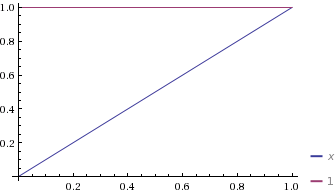
\includegraphics[width=0.5\linewidth]{/home/hellon/Dropbox/clientes/ana/images/5-a.png}
			\end{figure}

			Conforme sugestão do enunciado, considerando a imagem acima, podemos inverter a ordem de integração da seguinte forma

			$$\int _{0}^{1}\int _{0}^{x}e^{x^{2}}dydx$$

			Resolvendo a integral com relação a variavel $y$,

			$$\int _{0}^{1}ye^{x^{2}}\biggr\rvert_{0}^{x}dx = \dfrac{e^{x^{2}}}{2}\biggr\rvert_{0}^{1} = \dfrac {e-1}{2} $$

		\subsection*{Item b}

		O domínio da da integral em questão pode ser dado pela figura abaixo


		\begin{figure}[!ht]
			\centering
			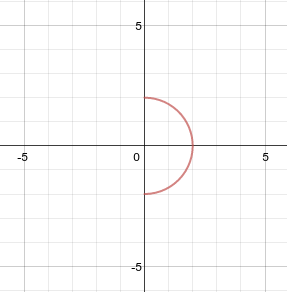
\includegraphics[width=0.4\linewidth]{/home/hellon/Dropbox/clientes/ana/images/5-b.png}
		\end{figure}

		Dado que estamos diante de um domínio circular, podemos rescrevê-lo da seguinte forma

		$$ D=\left\{ \left( r,\theta \right) \in \mathbb{R} ^{2} / 0\leq r\leq 2 \quad \textrm{e} \quad \dfrac {-\pi } {2}\leq \theta \leq \dfrac {\pi } {2}\right\} $$

		Reescrevemos nossa integral, pois, da seguinte forma

		$$\int _{-\frac {\pi } {2}}^{\frac {\pi } {2}}d\theta \int _{0}^{2}e^{-r^{2}}rdr$$

		Calculando...

		$$\int _{-\frac {\pi } {2}}^{\frac {\pi } {2}}d\theta \int _{0}^{2}e^{-r^{2}}rdr = - \left(\dfrac{e^{-r^{2}}}{2}\biggr\rvert_{0}^{2}\right) \pi = \dfrac{\pi}{2}(1-e^{-4})$$

		\subsection*{Item c}

		O domínio da da integral em questão pode ser dado pela figura abaixo

		\begin{figure}[!ht]
			\centering
			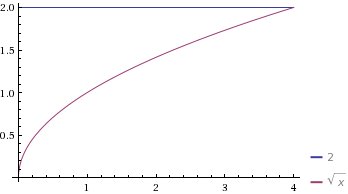
\includegraphics[width=0.5\linewidth]{/home/hellon/Dropbox/clientes/ana/images/5-c.png}
		\end{figure}

		Perceba então que podemos escrever a integral da seguinte forma

		$$\int _{0}^{2} \int _{0}^{y^2} \cos\left(y^3 \right) dxdy$$

		Calculando...

		$$\int _{0}^{2} \int _{0}^{y^2} \cos\left(y^3 \right) dxdy =  \int _{0}^{2} x\cos\left(y^3 \right)\biggr\rvert_{0}^{y^2} dy  = \int _{0}^{2} y^2\cos\left(y^3 \right) dy =  \dfrac {\sin(y^3)}{3} \biggr\rvert_{0}^{2} = \dfrac {\sin(8)}{3}$$



\end{document}
